%%%%%%%%%%%%%%%%%%%%%%%%%%%%%%%%%%%%%%%%%
% Short Sectioned Assignment
% LaTeX Template
% Version 1.0 (5/5/12)
%
% This template has been downloaded from:
% http://www.LaTeXTemplates.com
%
% Original author:
% Frits Wenneker (http://www.howtotex.com)
%
% License:
% CC BY-NC-SA 3.0 (http://creativecommons.org/licenses/by-nc-sa/3.0/)
%
%%%%%%%%%%%%%%%%%%%%%%%%%%%%%%%%%%%%%%%%%

%----------------------------------------------------------------------------------------
%	PACKAGES AND OTHER DOCUMENT CONFIGURATIONS
%----------------------------------------------------------------------------------------

\documentclass[paper=a4, fontsize=11pt]{scrartcl} % A4 paper and 11pt font size

\usepackage[T1]{fontenc} % Use 8-bit encoding that has 256 glyphs
\usepackage{fourier} % Use the Adobe Utopia font for the document - comment this line to return to the LaTeX default
\usepackage[english]{babel} % English language/hyphenation
\usepackage{amsmath,amsfonts,amsthm} % Math packages

\usepackage{minted} % Allows to put our code :)
\usepackage{graphicx} % Allows to put images :)
\usepackage[usenames, dvipsnames]{color} % Allows to have color :)
\usepackage{tikz} % Used for drawing state machines
\usepackage{pgf} % Used for drawing state machines
\usetikzlibrary{automata, positioning}
\usetikzlibrary{arrows}

\usepackage{sectsty} % Allows customizing section commands
\allsectionsfont{\centering \normalfont\scshape} % Make all sections centered, the default font and small caps

\usepackage{fancyhdr} % Custom headers and footers
\pagestyle{fancyplain} % Makes all pages in the document conform to the custom headers and footers
\fancyhead{} % No page header - if you want one, create it in the same way as the footers below
\fancyfoot[L]{} % Empty left footer
\fancyfoot[C]{} % Empty center footer
\fancyfoot[R]{\thepage} % Page numbering for right footer
\renewcommand{\headrulewidth}{0pt} % Remove header underlines
\renewcommand{\footrulewidth}{0pt} % Remove footer underlines
\setlength{\headheight}{13.6pt} % Customize the height of the header

\numberwithin{equation}{section} % Number equations within sections (i.e. 1.1, 1.2, 2.1, 2.2 instead of 1, 2, 3, 4)
\numberwithin{figure}{section} % Number figures within sections (i.e. 1.1, 1.2, 2.1, 2.2 instead of 1, 2, 3, 4)
\numberwithin{table}{section} % Number tables within sections (i.e. 1.1, 1.2, 2.1, 2.2 instead of 1, 2, 3, 4)

\setlength\parindent{0pt} % Removes all indentation from paragraphs - comment this line for an assignment with lots of text

%----------------------------------------------------------------------------------------
%	TITLE SECTION
%----------------------------------------------------------------------------------------

\newcommand{\horrule}[1]{\rule{\linewidth}{#1}} % Create horizontal rule command with 1 argument of height

\title{
\normalfont \normalsize
\textit{In The Name of God} \\
\textsc{Computer Engineering Department of Amirkabir University of Technology} \\ [25pt]
\horrule{0.5pt} \\[0.4cm] % Thin top horizontal rule
\huge Design Automation Homework - 3 \\ % The assignment title
\horrule{2pt} \\[0.5cm] % Thick bottom horizontal rule
}

\author{Iman Tabrizian (9331032)}

\date{\normalsize\today}

\begin{document}

\maketitle

%------- P5

\section{Problem 5}
%\center\includegraphics[]{p5.png}
\inputminted{vhdl}{q5/src/counter.vhd}
\par No of states, in state machine is equal to 18. For each number we have a
seperate state

\section{Problem 6}
%\center\includegraphics[]{p5.png}
\inputminted{vhdl}{q6/src/fsm.vhd}

\section{Problem 7}
%\center\includegraphics[]{p5.png}
\inputminted{vhdl}{q7/src/fsm.vhd}
\par From the benefits of this encoding is that the number of FFs are minimum
and disadvantage of this method is that if a noise occurs it's more difficult
to detect it.

\section{Problem 8}
\par You can find the state machine in the attachments
\inputminted{vhdl}{q8/src/averager.vhd}
\par Below is the figure of simulation result:
\center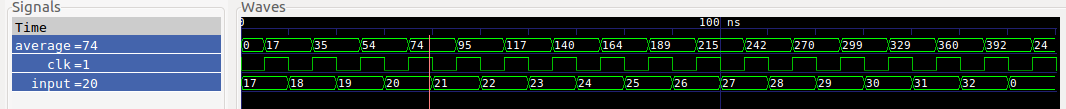
\includegraphics[scale=0.4]{q8.png}

\section{Problem 9}
\par You can find the state machine in the attachments
\center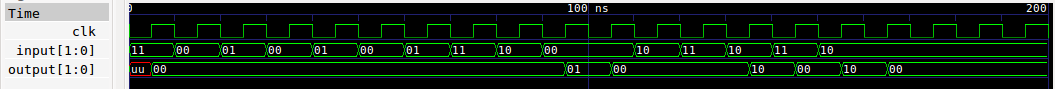
\includegraphics[scale=0.4]{q9.png}
\inputminted{vhdl}{q9/src/sequence_detector.vhd}

%\begin{tikzpicture}[->,>=stealth',shorten >=1pt,auto,node distance=2cm,
%                    semithick]
%   \node[state,initial] (q_0)   {$q_0$};
%   \node[state] (q_1) [right of=q_0] {$q_1$};
%   \node[state] (q_2) [right of=q_1] {$q_2$};
%   \node[state](q_3) [right of=q_2] {$q_3$};
%   \node[state](q_4) [right of=q_3] {$q_4$};
%   \node[state](q_5) [right of=q_4] {$q_5$};
%   \node[state](q_6) [right of=q_5] {$q_6$};
%   \node[state](q_7) [right of=q_6] {$q_7$};
%   \node[state](q_8) [below of=q_7] {$q_8$};
%   \node[state](q_9) [below of=q_6] {$q_9$};
%   \node[state](q_10) [below of=q_3] {$q_{10}$};
%   \node[state](q_11) [below of=q_2] {$q_{11}$};
%   \node[state](q_12) [below of=q_1] {$q_{12}$};
%   \path[->]
%   (q_0) edge [loop above] node {C, T} ()
%     edge [bend right] node [swap] {G} (q_1)
%     edge [bend right] node [swap] {A} (q_12)
%   (q_1) edge [loop below] node {G} ()
%     edge [bend left] node [swap] {A} (q_2)
%     edge [bend right] node {C, T} (q_0)
%   (q_2) edge [bend right] node {T} (q_3)
%     edge [bend right] node [swap] {C} (q_0)
%     edge [bend right] node {A} (q_12)
%     edge [bend right] node [swap] {G} (q_11);
   %(q_1) edge [bend right] node {0} (q_0)
   %  edge [bend right] node [swap] {1} (q_2)
   %(q_2) edge [bend right] node {0} (q_0)
   %  edge [bend right] node [swap] {1} (q_3)
   %(q_3) edge [bend right] node {0} (q_7)
   %  edge [bend right] node [swap] {1} (q_16)
   %(q_16) edge [bend left] node {0} (q_0)
   %  edge [loop below] node [swap] {1} ()
   %(q_7) edge [bend right] node {1} (q_6)
   %  edge [loop below] node {0} ()
   %(q_6) edge [bend right] node {1} (q_5)
   %  edge [bend right] node {0} (q_7)
   %(q_5) edge [bend right] node {1} (q_4)
   %  edge [bend right] node {0} (q_7)
   %(q_4) edge [bend left] node {1} (q_17)
   %  edge [bend right] node {0} (q_8)
   %(q_17) edge [bend left] node {0} (q_7)
   %  edge [loop below] node [swap] {1} ()
   %(q_8) edge [loop above] node {0} ()
   %  edge [bend right] node [swap] {1} (q_9)
   %(q_9) edge [bend right] node {0} (q_8)
   %  edge [bend right] node [swap] {1} (q_10)
   %(q_10) edge [bend right] node {0} (q_8)
   %  edge [bend right] node [swap] {1} (q_11)
   %(q_11) edge [bend right] node {0} (q_15)
   %  edge [bend right] node [swap] {1} (q_18)
   %(q_18) edge [bend right] node {0} (q_8)
   %  edge [loop below] node [swap] {1} ()
   %(q_15) edge [bend right] node {1} (q_14)
   %  edge [loop below] node {0} ()
   %(q_14) edge [bend right] node {1} (q_13)
   %  edge [bend right] node {0} (q_15)
   %(q_13) edge [bend right] node {1} (q_12)
   %  edge [bend right] node {0} (q_15)
   %(q_12) edge [bend left] node {1} (q_19)
   %  edge [bend right] node {0} (q_20)
   %(q_19) edge [bend left] node {0} (q_15)
   %  edge [loop below] node [swap] {1} ()
   %(q_20) edge [loop above] node {0,1} ();
%\end{tikzpicture}

\section{Problem 10}
%\center\includegraphics[]{p5.png}
\inputminted{vhdl}{q7/src/fsm.vhd}
\par We used only one process.
\end{document}
